\documentclass{article}
\usepackage[english]{babel}
\usepackage[utf8]{inputenc}
\usepackage{graphicx}
\usepackage{rotating}
\usepackage{hyperref}

\begin{document}
\title{Report for the Project	``Supervised Learning of Basis Function 
Coefficients for Computer-generated Speech''}
\date{\today}
\author{Franz Papst}
\maketitle

\section{Introduction}
The project ``Supervised Learning of Basis Function Coefficients for 
Computer-generated Speech'' was about trying a novel approach for speech 
synthesis by representing spectral parameters, used for speech synthesis, as 
weighted sums of basis functions. The obtained coefficients are then used for 
training a machine learning model which is then used for predicting the 
coefficients for test files. The predicted coefficients are used for 
recomposing the spectral parameters and generating an audio file from this 
recomposed spectral parameters and are plotted to have a visual representation 
of the values and to easily compare them with the original values.

\section{Implementation of the Project}
The project was implemented using the Python programming language. It offers a 
multitude of open libraries for scientific computing and for machine learning. 
In this project NumPy \cite{numpy}, Matplotlib \cite{matplotlib} and 
scikit-learn \cite{scikit-learn} were used. For synthesising the speech signal 
the Speech Signal Processing Toolkit \cite{sptk} was used.

As test and training data the CMU\_ARCTIC databases \cite{CMU_arctic} as 
provided by the HMM-based Speech Synthesis System Demo \cite{hts} were used.

\subsection{Steps for training a Model}
\begin{itemize}
	\item Identifying all phones in the training set.
	\item Converting the phones into numerical values.
	\item Encoding all training files as basis function coefficients.
	\item Training the model, using the numerical phone values as $\mathbf{X}$ 
	matrix and the coefficients as $\mathbf{y}$ matrix.
\end{itemize}

\subsection{Steps for testing a Model}
\begin{itemize}
	\item Predict the basis function coefficients using a trained model.
	\item Assigning the basis function coefficients to a basis function 
	coefficients representation instance and use this instance to produce audio 
	files and plot the predicted spectral parameters.
\end{itemize}

\section{Results}
\subsection{Encoding using different numbers of Basis Functions}
\begin{figure}
	\centering
	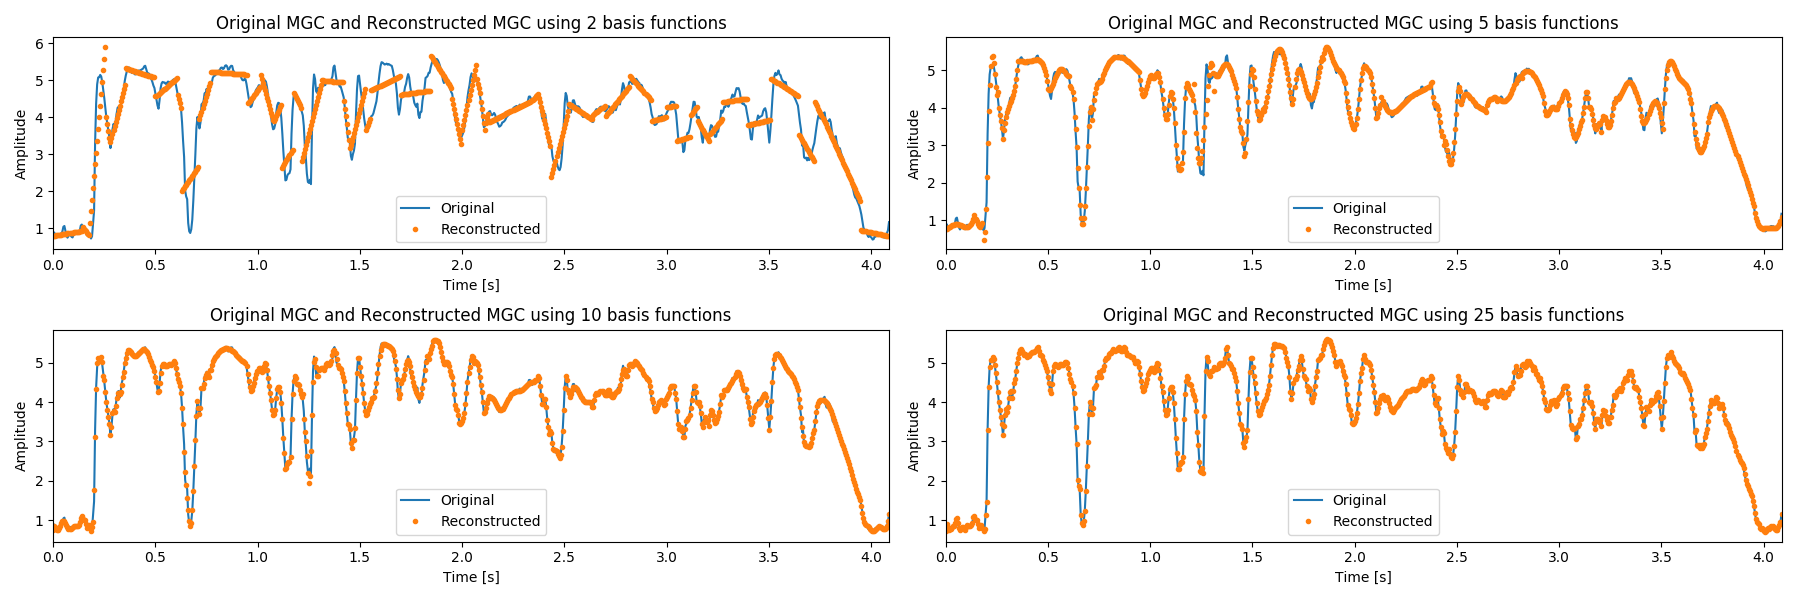
\includegraphics[width=\linewidth]{different_basis_functions}
	\caption{Different numbers of basis functions used for encoding the mel 
	generalised cepstral coefficients (MGC).}
	\label{different_basis_functions}
\end{figure}

Figure \ref{different_basis_functions} shows the encoding of the mel 
generalised cepstral coefficients (MGC) using four different (2, 5, 10 and 
25) basis functions to encode the MGC values. Legendre polynomials are used for 
encoding the MGC values. The plots show that encoding the MGC values using only 
two basis functions leads to a distorted result when the values are decoded. 
Using 5 basis functions to encode the MGC values already leads to a result that 
closely resembles the original matrix. Using 10 or 25 basis functions to encode 
the MGC values leads to even better results, although in the produced audio 
files the difference is not really noticeable. Also the difference in the plots 
of 10 and 25 basis functions is so small that it is negligible.

Based on this findings 5 basis functions were used for encoding, because it 
offers a sufficient representation of the original values while not using too 
much resources.

\subsection{Predictions of Spectral Parameters}
\begin{sidewaysfigure}
	\centering
	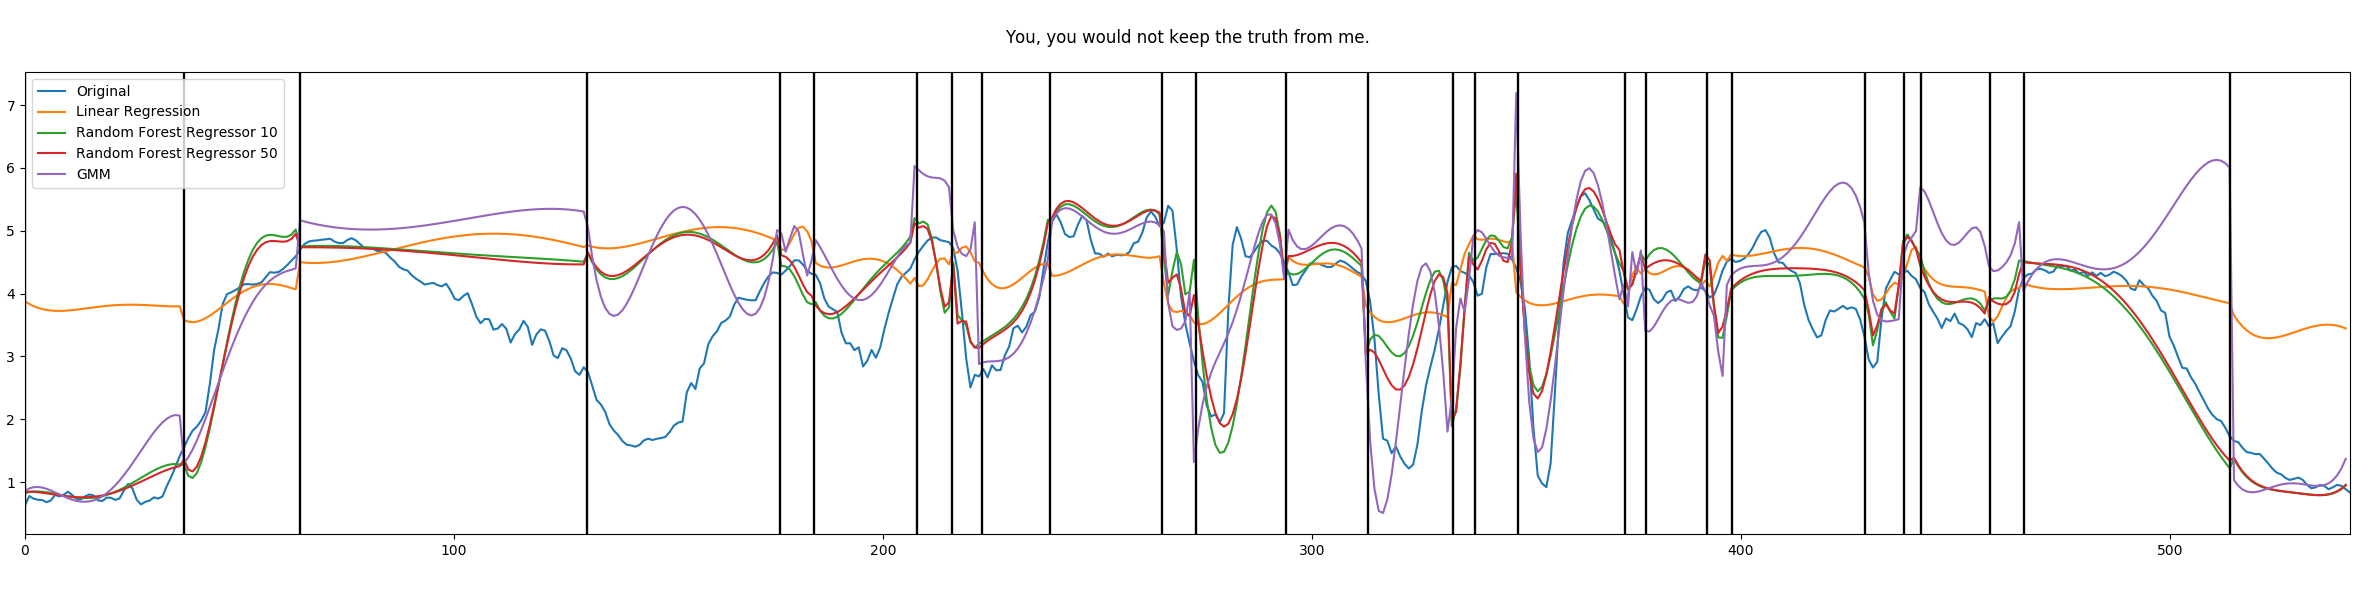
\includegraphics[height=6cm,keepaspectratio]{cmu_us_arctic_slt_a0101}
%TODO enter text
	\caption{The result of different models for predicting the first line of MGC 
	values for the phones in the sentence ``You, you would not keep the truth 
	from me.''}
	\label{prediction1}
\end{sidewaysfigure}

\begin{sidewaysfigure}
	\centering
	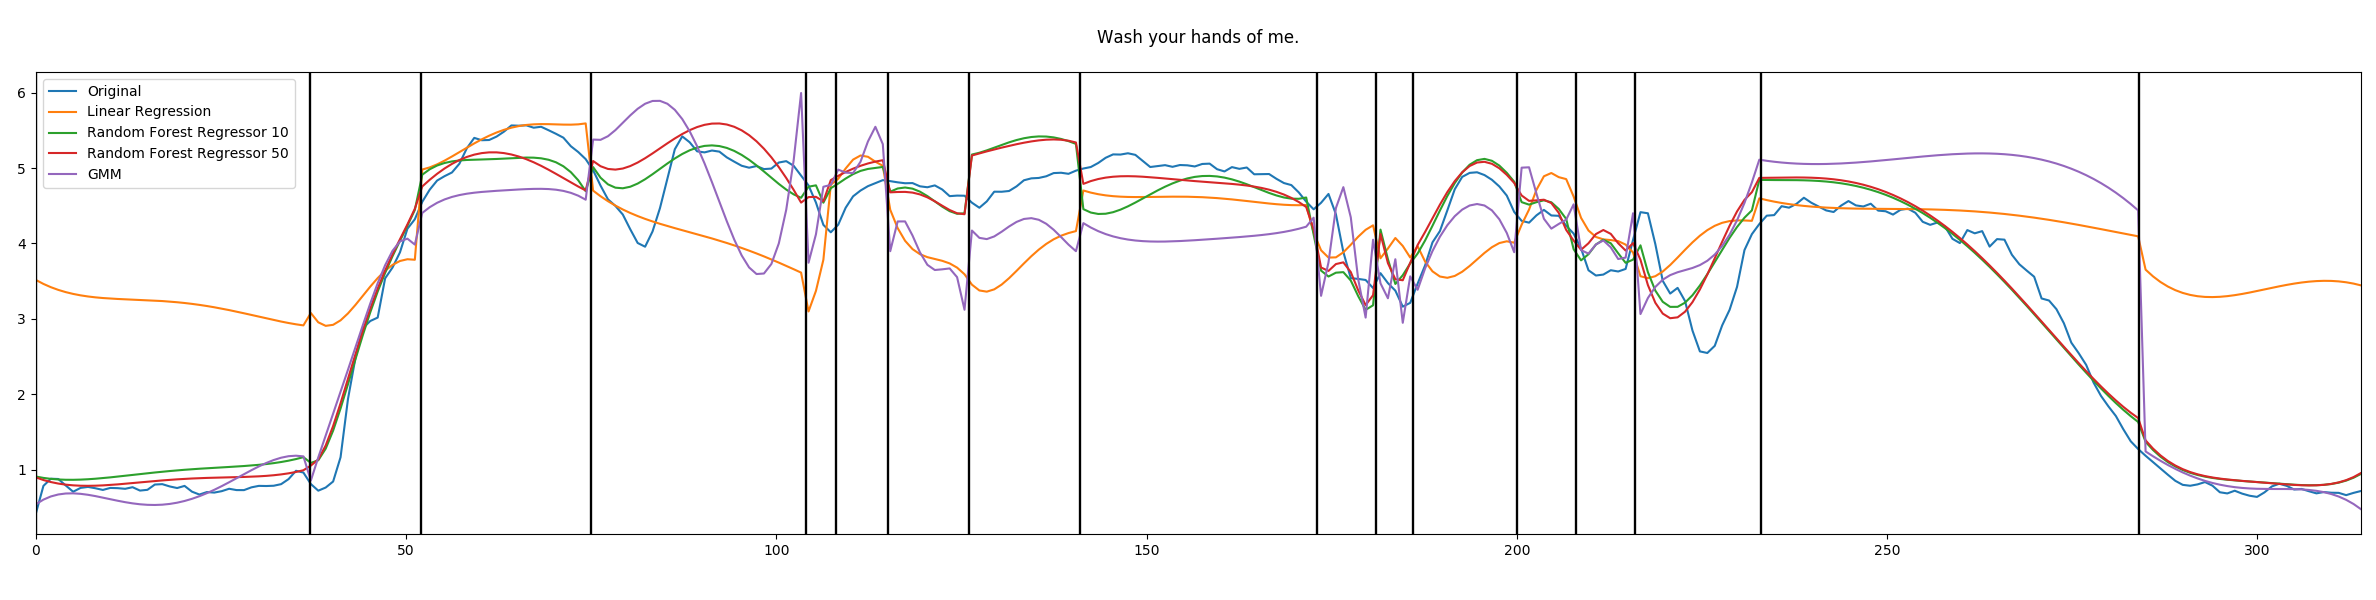
\includegraphics[height=6cm,keepaspectratio]{cmu_us_arctic_slt_a0240}
%TODO enter text
	\caption{The result of different models for predicting the first line of MGC 
	values for the phones in the sentence ``Wash your hands of me.''}
	\label{prediction2}
\end{sidewaysfigure}

Figures \ref{prediction1} and \ref{prediction2} show two examples of predicted 
MGC values done by different models. In both examples a random forest regressor 
gives the best results. For figure \ref{prediction1} the random forest 
regressor with 10 trees and the random forest regressor with 50 trees give 
almost the same prediction. For figure \ref{prediction2} this is true for parts 
of the prediction, but around an x-value of 150 the random forest regressors 
gave different values and the one with 50 trees gives the more truthful 
prediction. In general the random forest regressor with 50 trees gives better 
results, but has also more performance requirements (especially memory). The 
produced audio files for regressors with 10 and 50 trees are very similar to 
each other and are hardly distinguishable.

The predictions by the hierarchical Gaussian mixture model (HGMM)\footnote{A 
hierarchical Gaussian mixture model is a Gaussian mixture model with different 
layers for different combinations of phones: for a given quin-phone the model 
first looks up if there is the same quin-phone in the training data, if so a 
sample is drawn, if not the model looks up if a trained tri-phone (with the 
central phones of the previous quin-phone) is available, if so a sample is 
drawn, if not it draws a sample for the single-phone  (the one which is in the 
centre).} are not as good as the ones made by the random forest regressor, in 
both figures it the predictions made by the HGMM are vastly off the real values 
for some phones. In the produced audio file it is noticeable that the quality 
of the predictions is not as good as for the random forest regressor, audio 
files produced by the HGMM have the tendency to overdrive for some phones.

Both figures also show that linear regression is not really applicable for this 
problem. Especially at the beginning and at the end of the plots the results 
from linear regression are far off the real values. The prediction result is 
very smooth, so it is not able to capture the rapid changes of the original 
values (e.g. as show in figure \ref{prediction1} between the x-values of 300 
and 400).

\section{Conclusion}
Spectral parameters used for resynthesis of human speech can be represented as 
sum of basis functions, using 5 such basis functions is enough to resynthesise 
a file without noticeable quality loss.

The coefficients of these basis functions were used to train machine learning 
models on the phones they represent in order to make predictions for given 
phones. Random forest regressors have shown to give the best performance 
compared to a hierarchical Gaussian mixture model or linear regression. A HGMM 
still has superior performance compared with linear regression, but the 
produced audio files have the tendency to overdrive.

Due to the highly non-linear nature of the problem future research on the topic 
could be done using neural network, especially deep neural networks.

\bibliography{bibliography}
\bibliographystyle{IEEEtran}

\end{document}